\section{Durchführung}
\label{sec:Durchführung}

\subsection{Versuchsaufbau}
\label{sec:Versuchsaufbau}
%\begin{figure}
%	\centering
%	\caption{Schematische Darstellung des Versuchsaufbaus \cite{anleitung}.}
%	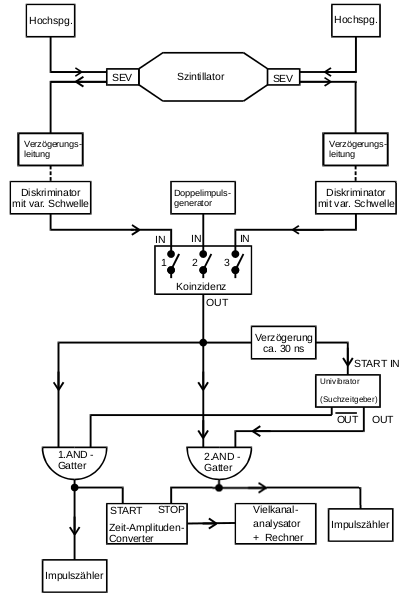
\includegraphics{Bilder/aufbau.png}
%	\label{fig:aufbau}
%\end{figure}
%
%\begin{figure}
%	\centering
%	\caption{Schematische Darstellung der Quelle zur Erzeugung radioaktiven Isotopen \cite{anleitung}.}
%	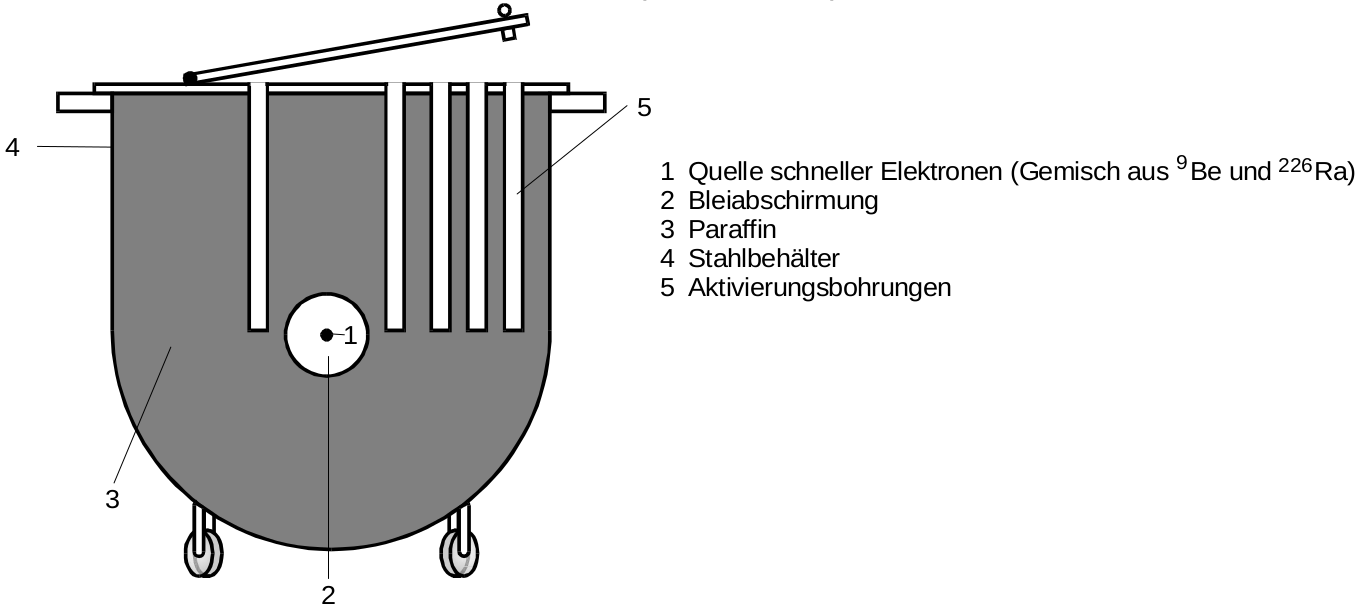
\includegraphics{content/toepfchen.png}
%	\label{fig:kochen}
%\end{figure}
%
Der Versuchsaufbau -- wie in Abbildung \ref{fig:aufbau} dargestellt -- besteht im Wesentlichen 
aus einem zerfallenden radioaktiven Isotop und einem Geiger-Müller-Zählrohr, welches die 
zerfallenden Kerne misst.
Das Geiger-Müller-Zählrohr ist entspricht einer mit Gas gefüllten Röhre. Trifft ein $\beta$-
oder $\gamma$- Teilchen auf ein Gasteilchen wird dieses ionisiert und kann aufgrund einer
anliegenden Spannung an der Röhre gemessen werden.
Dabei werden die gemessenen Zerfälle pro Messzeitintervall, welches am Zeitgeber einstellbar 
ist, an den Zählern 1 und 2 angezeigt. Nach jedem Messvorgang wird der Zähler umgeschaltet und 
der vorherige Wert auf dem aktuellen Zähler wird überschrieben. Der Versuchsaufbau ist mit
einer Blei-Abschirmung ausgestattet um die radioaktive Strahlung abzuschirmen.

Zur Erzeugung der radioaktiven Isotope wird das Objekt in Abbildung \ref{fig:kochen} verwendet.
Hierbei werden stabile Kerne mit niederenergetischen Neutronen beschossen. 
Da die Neutronen ihre Energie durch elastische Stöße an die Kerne übergeben und die maximale
Energie bei gleichen Massen der Stoßpartner erreicht wird, werden die Neutronen in einem 
Paraffinmantel gebremst, bis sie die optimale Energie besitzen.


\subsection{Versuchsbeschreibung}
\label{sec:Versuchsbeschreibung}
Vor Beginn der Messung muss ein möglichst scharfes Bild am Eintrittsspalt der Photozelle erzeugt werden.\\
Dazu wird direkt vor dem Eintrittsspalt eine Mattscheibe angebracht und die Positionen der optischen Elemente zueinander so variiert, dass ein scharfes Bild möglichst großer Intensität entsteht.\\
Mithilfe des Schwenkarms wird die Photozelle so ausgerichtet, dass nur monochromatisches Licht, also einfarbiges Licht mit nur einer Wellenlänge, auf den Eintrittsspalt der Photozelle fällt.\\
Die anliegende variable Gegenspannung wird schrittweise erhöht, bis kein Photostrom mehr am Piktometer abgelesen wird. Es werden etwa 10-15 Datenpaare aus angelegter Gegenspannung und Photostrom notiert.\\
Ebenso wird mit allen Spektrallinien verfahren, welche zu Beginn auf der Mattscheibe sichtbar waren.\\
Für niedrige Photoenergien, also recht langwelliges Licht, kann es nötig sein, ebenso beschleunigte Spannungen anzulegen, um eine genügend große Anzahl an Datenpaaren aus Spannung und Photostrom aufnehmen zu können.\\
Anschließend wird für die Spektrallinie $\lambda=\SI{578}{\nano\meter}$, also gelbes Licht, sowohl mit beschleunigendem als auch bremsenden Potential der Photostrom gemessen.
Die angelegte Spannung wird hierfür von $U=\SI{+20}{\volt}$ als beschleunigendes Potential bis zum bremsenden Potential, bei welchem der Photostrom verschwindet, gemessen.
Es werden etwa 40 Datenpaare aus anliegendem Potential und dem Photostrom notiert.
